\documentclass[a4paper, twoside]{report}

%% Language and font encodings
\usepackage[english]{babel}
\usepackage[utf8x]{inputenc}
\usepackage[T1]{fontenc}

%% Sets page size and margins
\usepackage[a4paper,top=3cm,bottom=2cm,left=3cm,right=3cm,marginparwidth=1.75cm]{geometry}

%% Useful packages
\usepackage{amsmath}
\usepackage{graphicx}
\usepackage[colorinlistoftodos]{todonotes}
\usepackage[colorlinks=true, allcolors=blue]{hyperref}

\title{Wave Propagation in Periodic Lattices}
\author{Bernard Ting}

\begin{document}
\begin{titlepage}

\newcommand{\HRule}{\rule{\linewidth}{0.5mm}} % Defines a new command for the horizontal lines, change thickness here

%----------------------------------------------------------------------------------------
%	LOGO SECTION
%----------------------------------------------------------------------------------------


\includegraphics[width=8cm]{title/logo.png}\\[1cm] % Include a department/university logo - this will require the graphicx package
 
%----------------------------------------------------------------------------------------

\center % Center everything on the page

%----------------------------------------------------------------------------------------
%	HEADING SECTIONS
%----------------------------------------------------------------------------------------

\textsc{\LARGE BEng Individual Project}\\[1.5cm] % Name of your university/college
\textsc{\Large Imperial College London}\\[0.5cm] % Major heading such as course name
\textsc{\large Department of Computing}\\[0.5cm] % Minor heading such as course title

%----------------------------------------------------------------------------------------
%	TITLE SECTION
%----------------------------------------------------------------------------------------
\makeatletter
\HRule \\[0.4cm]
{ \huge \bfseries \@title}\\[0.4cm] % Title of your document
\HRule \\[1.5cm]
 
%----------------------------------------------------------------------------------------
%	AUTHOR SECTION
%----------------------------------------------------------------------------------------

\begin{minipage}{0.4\textwidth}
\begin{flushleft} \large
\emph{Author:}\\
\@author % Your name
\end{flushleft}
\end{minipage}
~
\begin{minipage}{0.4\textwidth}
\begin{flushright} \large
\emph{Supervisor:} \\
Prof. Richard Craster \\[1.2em] % Supervisor's Name
\emph{Second Marker:} \\
Dr. Christopher Ford
\end{flushright}
\end{minipage}\\[2cm]
\makeatother

% If you don't want a supervisor, uncomment the two lines below and remove the section above
%\Large \emph{Author:}\\
%John \textsc{Smith}\\[3cm] % Your name

%----------------------------------------------------------------------------------------
%	DATE SECTION
%----------------------------------------------------------------------------------------

{\large \today}\\[2cm] % Date, change the \today to a set date if you want to be precise

\vfill % Fill the rest of the page with whitespace

\end{titlepage}


\begin{abstract}
We first introduce the theory of dispersion curves and plot them for simple
models. We then break the symmetry by introducing masses of different weights
and observe how this affects the dispersion curves. We then investigate their
structures in the case of mixed periodic structures and use this to find
special frequencies or modes which are present in the band gap. Scattering
simulations are run with these frequencies induced to the lattice to confirm
our analysis.
\end{abstract}

\renewcommand{\abstractname}{Acknowledgements}
\begin{abstract}
I would like to extend my greatest thanks to my supervisor, Prof. Richard Craster, for his advice and guidance on all matters relating to the project.
\end{abstract}

\tableofcontents
\listoffigures
\listoftables

\chapter{Introduction}
The study of metamaterials has the potential to solve many modern engineering problems.
\section{Objectives}
\section{Challenges}
\section{Contributions}

\chapter{Background}
Waves exhibit many characteristics when travelling through different media.
Much research has been carried out to investigate and harness these properties
to develop technologies and devices which manipulate electromagnetic (photonic)
and also acoustic (phononic) waves.

\section{History}
Since the earliest days of human history, we have sought to better understand
the natural world around us and so create technologies to improve our lives. At
first by utilising what nature already has to offer, but later on developing
materials and devices which have desirable properties not found in nature.

This progression describes roughly how the study of metamaterials came about.
It began in 1887 with the study of how certain crystals exhibit interesting
iridescence.\cite{pcearliest} After two independently developed landmark papers
were published in 1987 on structures with band gaps for electromagnetic
waves,\cite{pceli,pcjohn} the term photonic crystal --- a periodic optical
nanostructure which manipulates the passage of electromagnetic radiation ---
was coined.\cite{pcfocus} Since then, photonic crystals have been mass produced
and used for many purposes, e.g. optical fibres for transmission of digital
information \cite{pcopfib} and precision surgery.\cite{pcsurgery,pcneuro}

Then came the study of metamaterials --- materials engineered to possess some
property not found in naturally occurring materials.\cite{briefintro} Usually
these materials are composed of smaller units which are arranged in a repeating
pattern. They derive their properties not from the intrinsic properties of the
base materials, but from the periodic structure introduced.

One of the first major breakthroughs which the study of metamaterials led to
was the development of materials with a negative refractive index. Though the
possibility of creating such a material was theoretically predicted in
1967,\cite{negrefrac} it was only experimentally verified in
2001.\cite{negrefracex}

Nowadays, there is much research being done in the area of topological
metamaterials or topological photonic
crystals.\cite{topoedge,toposplit,topomet} This is where new properties of
metamaterials are produced by perturbing their structures utilising topological
and group theoretic concepts, usually by breaking symmetries which are present
in the original material. The reason there is considerable interest in applying
these abstract fields to the study of metamaterials is due to their ability to
transcend specific physical systems and be applied widely. An example is being
able to create metamaterials which split energy in multiple
directions.\cite{toposplit} Since then, much research has been done in
emulating these topological effects in simpler systems and then transferring
the results into proper experimentation in the desired
contexts.\cite{elasticvhe,singlevalley,exobs,exobs2} This forms an exciting
modern area of wave physics and we mention below some of the novel applications
which can be realised with these systems.

\section{Practical applications}
\label{applications}
Metamaterials have the potential to solve many modern engineering problems.

\begin{itemize}
\item Developing a cloak of invisibility.\cite{emcloak}
      \begin{itemize}
      \item Obvious use cases in military.
      \item Protect things from electromagnetic radiation.
      \end{itemize}
\item Constructing antennae to focus energy into narrow beams.
      \cite{diremi,antennasol}
      \begin{itemize}
      \item Gather wave energy from deep in the oceans and concentrate them to
            be harvested.
      \item Channel sound energy, e.g. from train tracks, to be dissipated
            elsewhere which decreases noise pollution.
      \end{itemize}
\item Producing devices which operate on the terahertz ($1THz=10^{12}Hz$)
      range.\cite{THz}
      \begin{itemize}
      \item Can be used in medical imaging due to terahertz radiation being
            able to penetrate thin materials but not thicker objects. Also, it
            is non-ionising radiation and so does not damage living cells
            unlike X-rays.
      \item For surveillance, especially security screening as many materials
            of interest have unique spectral fingerprints in the THz
            range.\cite{Thzsec}
      \end{itemize}
\item Developing near perfect electromagnetic absorbers.\cite{absorbing}
\item Developing energy splitters.\cite{toposplit}
\item Developing perfect lenses.\cite{negrefraclens}
\end{itemize}

\section{Models studied}
There are many different models which we can use to study the effects of
metamaterials on the waves which propagate through them. 

\begin{figure}[!h]
\centering
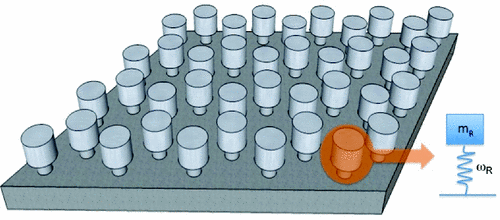
\includegraphics[width=0.8\textwidth]{imgs/flexplate.png}
\caption{\label{fig:flexplate} Schematic view of a thin plate flexural wave
         model which consists of an array of resonators attached to a thin
         elastic plate. Each resonator is a point mass attached to the plate by
         a spring. Image adapted from source.\cite{graphene}}
\end{figure}

In the literature, thin plate flexural wave theories,\cite{graff,toelastic} as
seen in Figure~\ref{fig:flexplate}, have proven to be highly effective physical
models and reliable predictors of physical wave phenomena as shown by the
numerous studies done on flexural (or bending) waves in a beam or a
plate.\cite{flexbeam,graphene,mehulgeom} This is very advantageous as most
acoustic (or sound) radiation travels as flexural waves through structures and
deforms the medium transversely as they propagate.\cite{sound} Therefore, these
models are very useful in studying acoustic metamaterials or phononic
crystals.\cite{phonon} As a specific example, an elastic analogue of graphene,
a honeycomb arrangement of mass-spring resonators attached to a thin elastic
plate, was shown which could be used as waveguides.\cite{graphene}

Having said that, the equations which govern the propagation of flexural waves
are much more complicated than those for a simple mass-spring system and
requires more background knowledge in its physics to properly understand and
implement. As an example, the biharmonic equation which governs the propagation
of flexural waves in a lattice of mass-spring resonators is a fourth-order
partial differential equation.

Along the same lines, the modelling of electromagnetic metamaterials present
the challenges of getting to grips with the theory of electromagnetic
radiation, e.g. Maxwell's equations\cite{maxwell} and Bragg
scattering\cite{bragg}.

\begin{figure}
\centering
  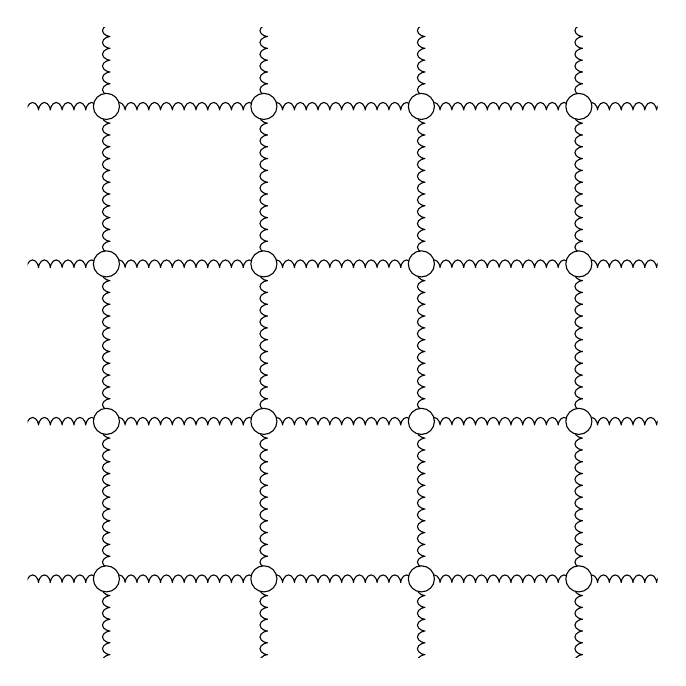
\begin{tikzpicture}
    \clip (-1,-1) rectangle (7,7);
    \foreach \X in {-2,0,...,6}
    {\foreach \Y in {-2,0,...,6}
     {\draw[decorate,decoration={coil,aspect=0.5,amplitude=0.5mm, segment
    length=1.5mm}] (\X,\Y) -- ++(0,2) -- ++(2,0);
    \node[circle,draw,inner color=white] at (\X,\Y) {};}}
  \end{tikzpicture}
  \caption{\label{fig:ourmodel} Schematic view of our simple mass-spring model.}
\end{figure}

Given the timeline of this project, the limited Physics background I have, as
well as to make the results accessible to a wider audience, we have decided to
go for a simplistic masses-connected-by-springs model, as seen in
Figure~\ref{fig:ourmodel}, as the core object of study in our project. The
lattice will be formed of repeating cells (e.g. Figure~\ref{fig:sqscheme}) and
it is the periodicity in the lattice which will give rise to its special
properties. Not only does this reduce the complexity as we only need to deal
with ordinary differential equations and not partial differential equations, it
also reduces the complexity in the scattering simulations as we now have to
solve a discrete system instead of a continuous one. With this \textit{toy}
system which form the basic building blocks of solid state physics, we will be
able to more quickly lay the foundations required to carry out more interesting
experiments, from which results can be transferred to other models.

The two lattices which we will be focusing most of this work on is the
hexagonal and kagome lattice. This is because they have a lot of physical
analogues which are particularly useful.\cite{singlevalley,wuandhu,kphysical}
As a concrete example, the kagome lattice shown in
Figure~\ref{fig:kagomescheme} has a physical analogue as a dense packed system
such as the one shown in Figure~\ref{fig:kagomephysical}. The dense packed
system consists of particles and voids filled with fluid connected by thin
gaps. The key to controlling the behaviour of the crystal is being able to
precisely engineer the thin gaps, as the gaps and voids together form a
connected network of resonators. Thus, it can be seen that our model is
asymptotically equivalent to this physical system.\cite{kphysical}

\begin{figure}[!h]
\centering
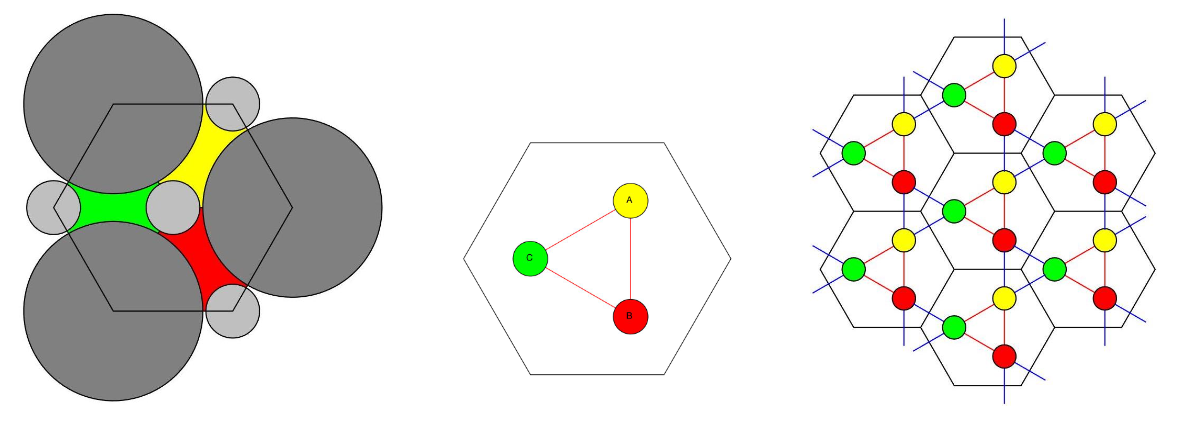
\includegraphics[width=0.8\textwidth]{imgs/kagomephysical.PNG}
\caption{\label{fig:kagomephysical} The closely packed system (left) shows
rigid cylindrical inclusions of two different radii, the elementary hexagonal
cell and the three voids (yellow, green, red) connected by thin gaps. The
asymptotically equivalent Kagome lattice as a discrete network model (right).
Image and caption adapted from source.\cite{kphysical}.}
\end{figure}

The following will be brief explanations of concepts which will form the
foundation on which we will analyse and investigate the properties of our
lattices.

\section{Dispersion relation}
\label{disperbg}
A dispersion relation relates the wavenumber of a wave to its frequency. We
will see that this relation is of utmost importance when discussing periodic
lattices as only waves of certain frequencies are transmitted by the lattice
and the dispersion relation directly shows us which frequencies these are. As
we will be solving for the dispersion relation of infinite and semi-infinite
lattices in Chapter \ref{disperrel} and \ref{perturbed}, we will be making use
of the concepts below to simplify the problem (because we do not want to solve
an infinite problem!).

\section{Bloch waves}
\label{blochbg}
Bloch's theorem for waves in a periodic potential\cite{bloch} states that any
wave travelling through a periodic potential can be expressed as the product of
a periodic function and a plane wave,\cite{kittel} i.e.

\begin{align}
  \psi_{\vec{\kappa}}(\vec{r})=f_{\vec{\kappa}}(\vec{r})e^{i\vec{\kappa}\cdot\vec{r}}
\label{eq:blochwave}
\end{align}

where $f_{\vec{\kappa}}(\vec{r})$ has the period of the lattice with
$f_{\vec{\kappa}}(\vec{r})=f_{\vec{\kappa}}(\vec{r}+\vec{R})$, with $\vec{R}$ being a
translation vector of the lattice.

The proof of this theorem can be found here.\cite{kittel} But we will just
state how we can use this result to simplify the equations we will obtain in
our systems. This is useful for us as we are modelling elastic waves travelling
through a periodically-repeating mass-spring system and so Bloch's theorem
applies. Thus we can write the displacement of one mass as the displacement of
another corresponding mass in the lattice with a complex exponential factor. By
doing this, we can characterise the behaviour of all the displacements by just
focusing on finding the displacements of masses in the \textit{primitive cell},
which is just the unit cell which forms the repeating base of our lattice. We
will see later how this helps to reduce our infinite system of equations down
to a finite number, such as in \eqref{eq:HLN2L} and \eqref{eq:blochsq}.

\section{Reciprocal lattice}
\label{reclatbg}
A reciprocal lattice represents the Fourier transform of another lattice. In
our case, our model lattice is a periodic spatial function in real space, and
so its reciprocal lattice exists as a function of frequency in reciprocal
space.  We will continue with a more formal explanation based on the materials
in the Appendix of this book,\cite{moldinglight} restricting our discussion to
only 2-dimensional lattices which is sufficient for our purposes.

More formally, suppose we have a function $f(\vec{r})$ which is periodic on a
lattice, i.e. $f(\vec{r})=f(\vec{r}+\vec{R})$ for all vectors $\vec{R}$
that translate the lattice onto itself (connect a lattice point to the next).
Then we call $\vec{R}$ the \textit{lattice vectors}. As we shall see later,
elastic waves travelling through our mass-spring lattices are examples of such
a periodic function. Naturally then, we would take the Fourier transform when analysing a periodic function, i.e.

\begin{align}
  f(\vec{r})=\int c\vec{q}g(\vec{q})e^{i\vec{q}\cdot\vec{r}}
\end{align}

Applying periodicity, we see that

\begin{align}
  &f(\vec{r}+\vec{R})=f(\vec{r}) \\
  &\Rightarrow\int c\vec{q}g(\vec{q})e^{i\vec{q}\cdot\vec{r}}e^{i\vec{q}\cdot\vec{R}}=\int c\vec{q}g(\vec{q})e^{i\vec{q}\cdot\vec{r}} \\
  &\Rightarrow g(\vec{q})=g(\vec{q})e^{i\vec{q}\cdot\vec{R}}
\end{align}

Therefore, this tells us that the transform $g(\vec{q})$ has to be zero
everywhere, except where $e^{i\vec{q}\cdot\vec{R}}=1$, or equivalently
$\vec{q}\cdot\vec{R}=2\pi N$ for any $N\in \mathbb{Z}$. These vectors $\vec{q}$ that
satisfy this condition are called the \textit{reciprocal lattice vectors} and
are usually designated by $\vec{G}$. Note also that these reciprocal lattice
vectors form a lattice of their own, which we can easily verify as

\begin{align}
(\vec{G}_1+\vec{G}_2)\cdot\vec{R}=\vec{G}_1\cdot\vec{R}+\vec{G}_2\cdot\vec{R}=2\pi (N_1+N_2)
\end{align}
 
and we call this reciprocal lattice the \textit{reciprocal space}.

So given a set of lattice vectors $\vec{R}$, to find the reciprocal lattice
vectors $\vec{G}$, we need to find all $\vec{G}$ such that
$\vec{G}\cdot\vec{R}$ is some integer multiple of $2\pi$ for every $\vec{R}$.
Since we know that $\{\vec{G}\}$ forms a lattice, we know that every reciprocal
lattice vector $\vec{G}$ can be written as $\vec{G}=l\vec{b_1}+m\vec{b_2}$ for
some set of primitive lattice vectors $\vec{b}_i$, similar to how any lattice
vector $\vec{R}$ can be written as $\vec{R}=p\vec{a_1}+q\vec{a_2}$ for some set
of primitive lattice vectors $\vec{a}_i$ which are the smallest vectors
pointing from one lattice point to another and need not be of unit length.
Therefore 

\begin{align}
  &\vec{G}\cdot\vec{R}=2\pi N \\
  &\Rightarrow (p\vec{a}_1+q\vec{a}_2)\cdot(l\vec{b}_1+m\vec{b_2})=2\pi N
\end{align}

From this, it is easy to see that constructing $\vec{b}_i$ such that
$\vec{a}_i\cdot\vec{b}_j=2\pi\delta_{ij}$ satisfies the above condition.
Therefore we see from this that if $\vec{a}_i$ is of length $a$, then
$\vec{b}_i$ will be of length $\frac{2\pi}{a}$, which is where the term
\textit{reciprocal} lattice is derived from.

\section{Brillouin zone}
\label{brizones}

The concept of Brillouin zones was first defined by Leon Brillouin in his book
on wave propagation in periodic structures.\cite{brillouin} As we are able to
tessellate our physical lattice with a periodically repeating unit cell, so
there exists a unit reciprocal cell which can cover the reciprocal space
without overlap. We will now motivate the selection of the first Brillouin zone
as a \textit{good} unit reciprocal cell based on the the discussions in
here.\cite{moldinglight}

To see how we might make a good choice for a unit cell for the reciprocal
space, notice that for the Bloch states (as defined in Chapter \ref{blochbg}),
different values of $\vec{\kappa}$ do not necessarily lead to different modes.
To be more precise, the modes with wave vector $\vec{\kappa}$ and
$\vec{\kappa}+2\pi N$ are identical, which means that $\vec{\kappa}$
essentially functions as the phase relationship between the displacement of
masses in our lattice. Now notice also that from \eqref{eq:blochwave} and the
fact that our lattice is periodic, we have that if $\vec{G}$ is a reciprocal
lattice vector (as defined in Chapter \ref{reclatbg}), then
$\vec{\kappa}+\vec{G}$ causes the phase difference between masses to be
incremented by $\vec{G}\cdot\vec{R}$ which we know is $2\pi N$ and so is no
difference at all!

This shows us that there is a lot of redundancy in $\vec{\kappa}$ and we do not
actually need to explore the whole of $\kappa$-space but it is enough for us to
restrict ourselves to a finite \textit{zone} in the reciprocal space from which
we \textit{cannot} get from one part of the lattice to area to another by
adding $\vec{G}$. This is visually demonstrated in Figure~\ref{fig:kappaspace}.

\begin{figure}[!h]
\centering
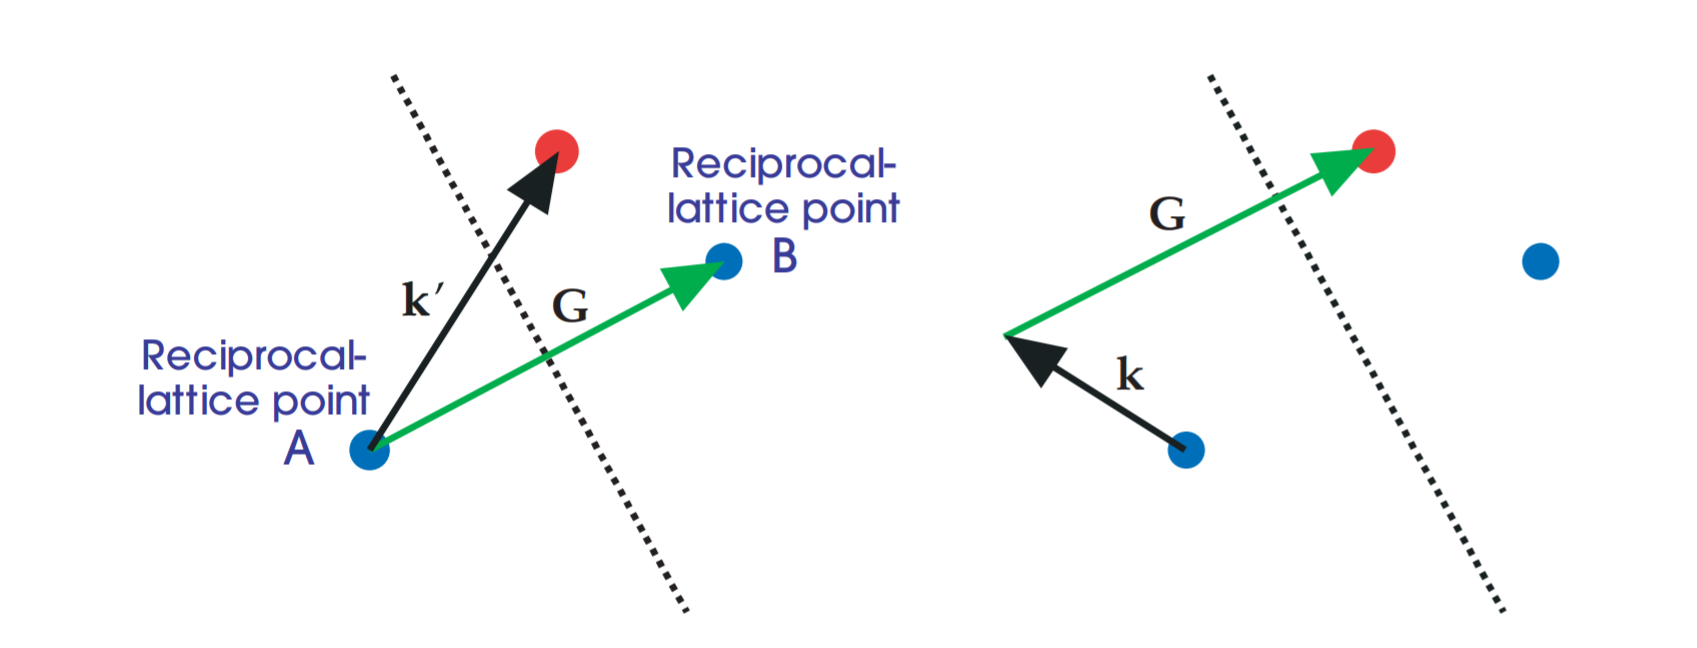
\includegraphics[width=0.8\textwidth]{imgs/kappaspace.PNG}
\caption{\label{fig:kappaspace} Characterisation of the Brillouin zone. The
  dotted line refers to the perpendicular bisector of the line joining two
  reciprocal lattice points (blue). Notice that if we choose the left point A
  as the origin, any lattice vector (such as $\vec{\kappa'}$) that reaches to
  an arbitrary point on the other side (red) can be expressed as the sum of a
  vector on the same side (such as $\vec{kappa}$) plus a reciprocal lattice
  vector $\vec{G}$. Image and caption adapted from source.\cite{moldinglight}.}
\end{figure}

There are many such zones, but we choose to focus on the region which is
closest to the origin, where $\vec{\kappa}=0$. And that zone is what we call
the first Brillouin zone. 

That is why the other way to define a Brillouin zone is that it is a particular
choice of this reciprocal cell and is constructed as the set of points enclosed
by the Bragg planes. The Bragg planes exist in reciprocal space and are the
planes perpendicular to a straight line from the origin to each lattice point.
The first Brillouin zone is then defined as the set of points formed by the
Bragg planes closest to the origin. These concepts are described visually for a
2d square real lattice in Figure~\ref{fig:bzonesq}.

The idea of Brillouin zones is brilliant in that now we know we only need to
solve for the dispersion relation for $\vec{\kappa}$ in the first Brillouin
zone to know the dispersion relation across the entire lattice.

\chapter{PROJECT X}
\chapter{Evaluation}
% TODO: Compare results to those of more complex models; look at other papers
% and use their parameters
As mentioned in Chapter \ref{applications}, most of the practical applications
of metamaterials and photonic crystals come from their ability to control the
propagation of acoustic or electromagnetic waves. As such, it is important to
evaluate our model in terms of whether the results can translate to other
complex models.

To evaluate the performance and accuracy of our mass-spring model, we will
therefore compare our results to those produced in other papers, some with the
mass-spring model and some with more complex continuous models.

\section{Further work}
% TODO: Can split into what we can do in terms of different perturbations/
% grading etc; but also look at computing side, e.g. split into classes so
% easier to run simulations and get dispersion curves etc
% - compare the two different kind of perturbations. Is there a difference?
% Alternating mass one seems to be better. Amplitude is higher
There are many things that we can improve on and continue investigating for the
future. 

In terms of investigating deeper the challenges that might be faced when going
from simulations to a real world product, the following could be useful:
\begin{itemize}
\item Evaluating the robustness of our system to imperfections in the lattice.
This is crucial as real production systems have certain tolerances and are not
perfect. As such, it is important to be able to test how little changes in the
lattice can affect the edge states that we get, in terms of the strength of the
energy which is transmitted as well as the amount of energy which is dissipated
throughout the lattice.

\item Testing how small each layer of material can be to get a \textit{good
enough} edge state. So far in our discussions of the strips of cells, we have
been using strips with a large number of cells (e.g. $2N=40$) because we know
that the edge states decay exponentially outwards from the boundary, but this
may not be possible or cost effective when developing real products. Therefore,
it is important to study how the number of cells translates to the amount of
energy lost and how this might lead to unwanted energy elsewhere in the system
or interference with our edge state along the boundary. An example can be seen
in Figure~\ref{fig:smallvsbig}.
\end{itemize}

\begin{figure}
\centering
\begin{subfigure}[b]{.5\textwidth}
  \centering
  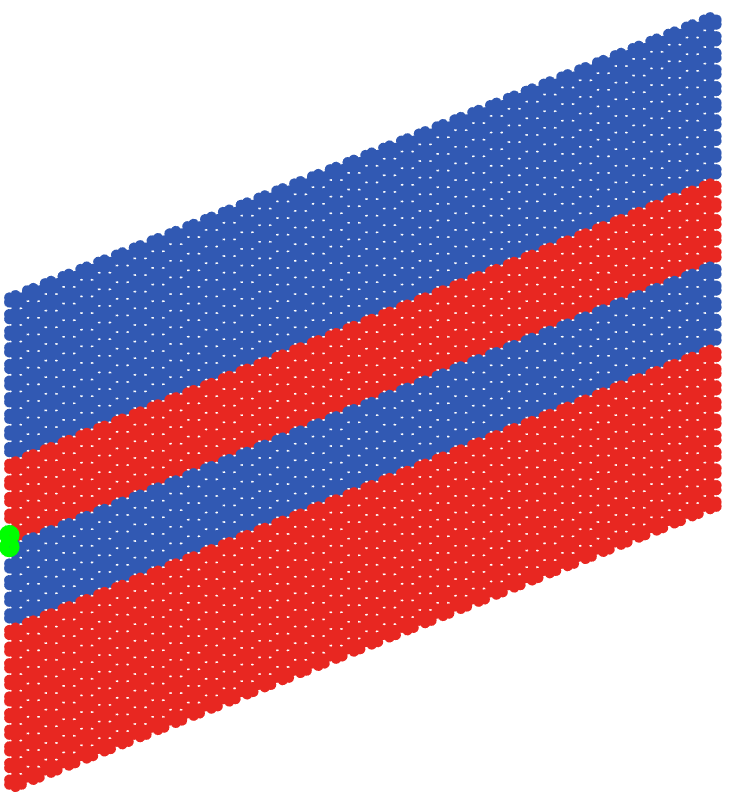
\includegraphics[width=0.7\linewidth]{imgs/svbthickarr.png}
  \caption{Arrangement of cells with $2N=10$.}
  \label{fig:sub1}
\end{subfigure}%
\begin{subfigure}[b]{.5\textwidth}
  \centering
  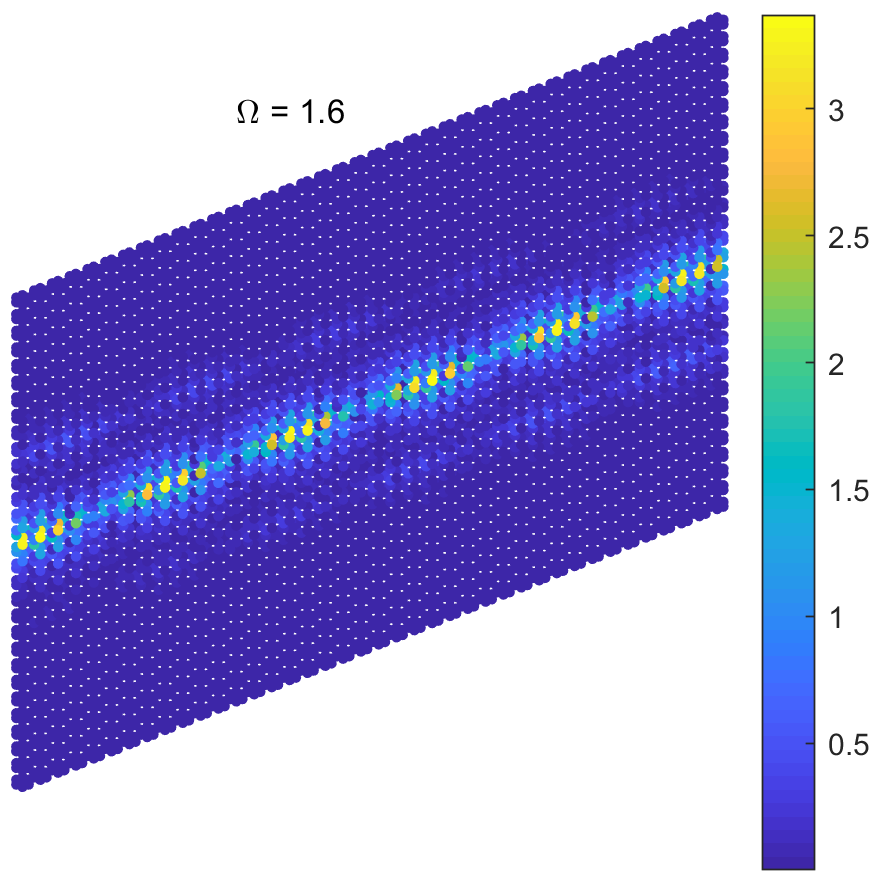
\includegraphics[width=0.9\linewidth]{imgs/svbthickscat.png}
  \caption{The plot of $|y_i|$ for each mass in each cell.}
  \label{fig:sub2}
\end{subfigure}

\medskip
\begin{subfigure}[b]{.5\textwidth}
  \centering
  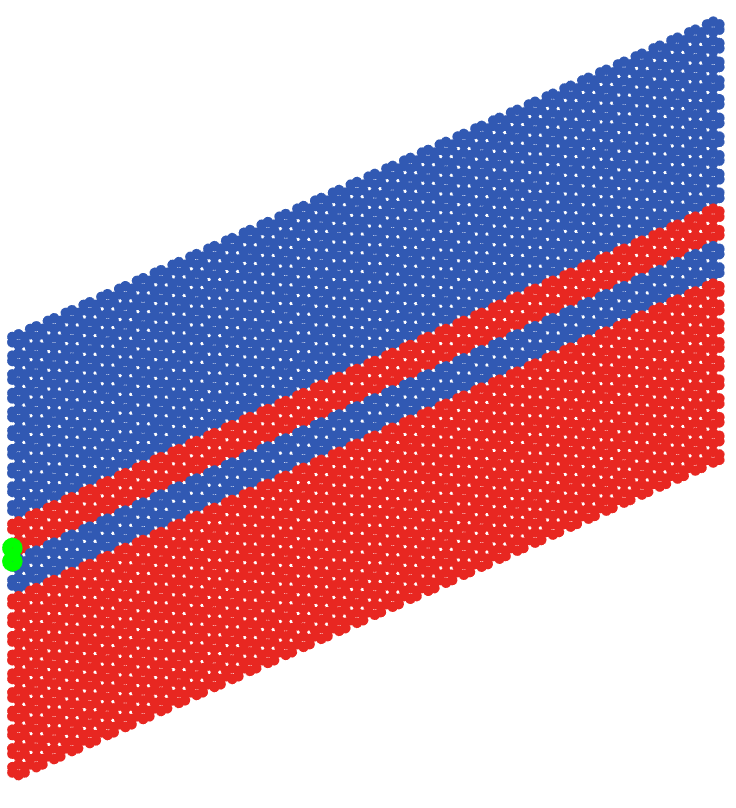
\includegraphics[width=0.7\linewidth]{imgs/svbthinarr.png}
  \caption{Arrangement of cells with $2N=4$.}
  \label{fig:sub1}
\end{subfigure}%
\begin{subfigure}[b]{.5\textwidth}
  \centering
  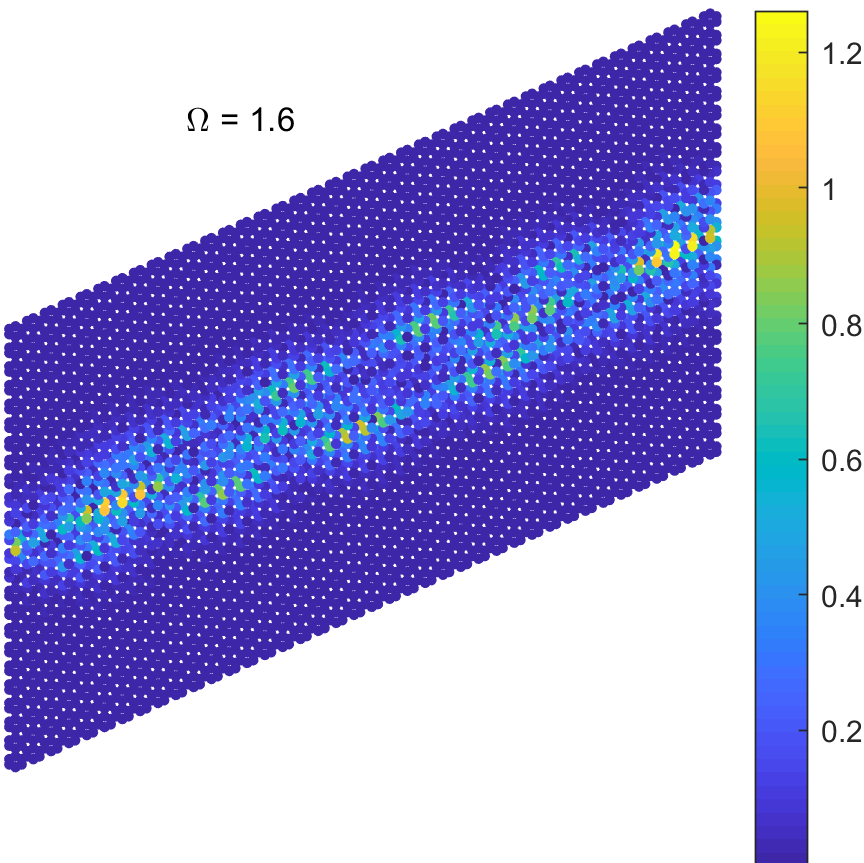
\includegraphics[width=0.9\linewidth]{imgs/svbthinscat.png}
  \caption{The plot of $|y_i|$ for each mass in each cell.}
  \label{fig:sub2}
\end{subfigure}

\medskip
\begin{subfigure}[b]{.5\textwidth}
  \centering
  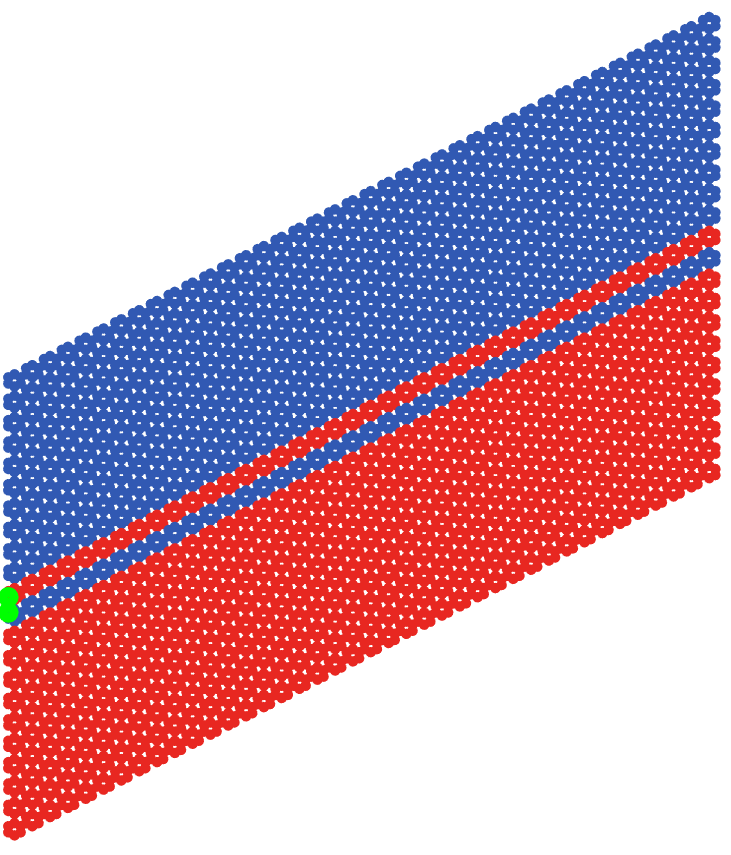
\includegraphics[width=0.7\linewidth]{imgs/svbthinnerarr.png}
  \caption{Arrangement of cells with $2N=2$.}
  \label{fig:sub1}
\end{subfigure}%
\begin{subfigure}[b]{.5\textwidth}
  \centering
  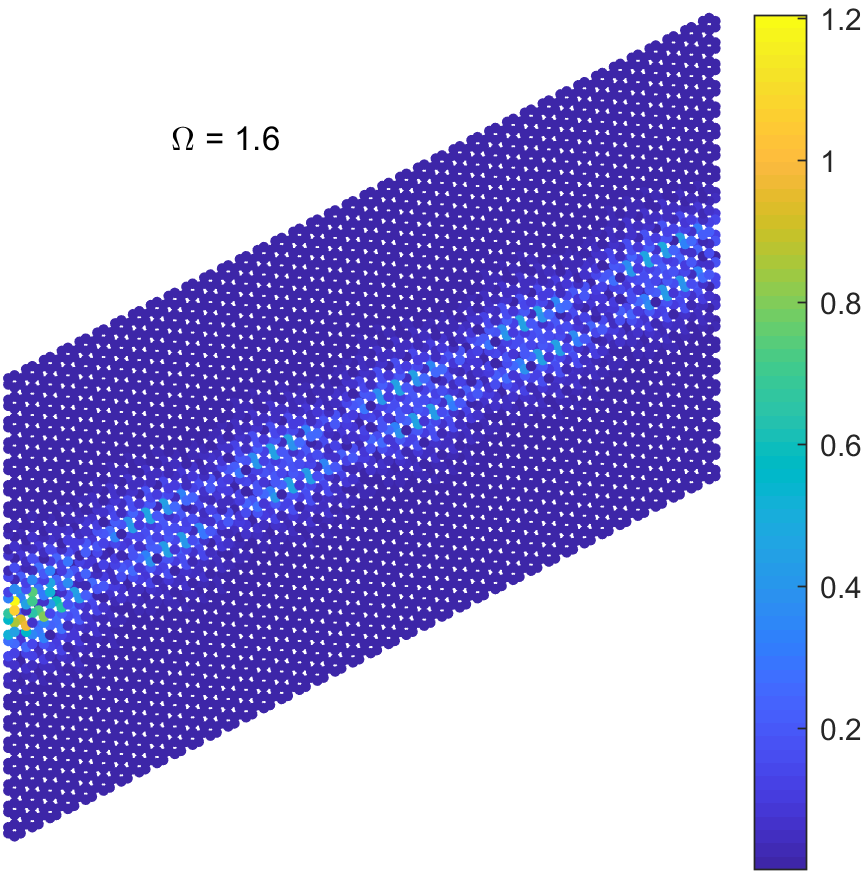
\includegraphics[width=0.9\linewidth]{imgs/svbthinnerscat.png}
  \caption{The plot of $|y_i|$ for each mass in each cell.}
  \label{fig:sub2}
\end{subfigure}
\caption{Scattering simulation to show the differences in amplitude and
  dissipation of energy for hexagonal boundaries of different thicknesses using
  the cells as defined in Figure~\ref{fig:hexstripMrotated}.}
\label{fig:smallvsbig}
\end{figure}

In terms of improving the workflow for the generation of these results for
other geometries and topologies, we could implement the following:
\begin{itemize}
\item Move to an object-oriented programming model. We can implement the
concepts of shapes and topologies as interfaces which contain information about
the required geometries. Then we can create specific classes corresponding to
actual shapes to extend those interfaces. We can then have our core code which
generates the dispersion relations and scattering simulations work based on the
interface implemented, rather than being specific to one shape class. This
should be relatively straightforward to implement, as most of the code to solve
for dispersion curves and scattering simulations is the same for any shape. The
only big difference for different topologies is the formation of the
eigen-problem matrix, which is a really mechanical but time-consuming
procedure, and so this will make testing out new shapes or different connection
of masses much easier.

\item To take the above idea and make it even more user-friendly, we could
create a graphical user interface where a user can choose things like the shape
of the cell, the position of masses within the cell and how the masses are
connected. This would allow faster and simpler prototyping of new designs.
\end{itemize}

\chapter{Conclusion}
\appendix
\chapter{First Appendix}

\bibliographystyle{alpha}
\bibliography{bibs/sample}

\end{document}
